\section{PRINT Print a Figure To A File}

\subsection{Usage}

This function ``prints'' the currently active fig to a file.  The 
generic syntax for its use is
\begin{verbatim}
  print(filename)
\end{verbatim}
or, alternately,
\begin{verbatim}
  print filename
\end{verbatim}
where \verb|filename| is the (string) filename of the destined file.  The current
fig is then saved to the output file using a format that is determined
by the extension of the filename.  The exact output formats may vary on
different platforms, but generally speaking, the following extensions
should be supported cross-platform:
\begin{itemize}
\item  \verb|jpg|, \verb|jpeg|  --  JPEG file 

\item  \verb|pdf| -- Portable Document Format file

\item  \verb|png| -- Portable Net Graphics file

\item  \verb|svg| -- Scalable Vector Graphics file

\end{itemize}
Postscript (PS, EPS) is supported on non-Mac-OSX Unix only.
Note that only the fig is printed, not the window displaying
the fig.  If you want something like that (essentially a window-capture)
use a seperate utility or your operating system's built in screen
capture ability.
\subsection{Example}

Here is a simple example of how the figures in this manual are generated.
@>
which creates two plots \verb|printfig1.png|, which is a Portable
Net Graphics file, and \verb|printfig1.jpg| which is a JPEG file.


\centerline{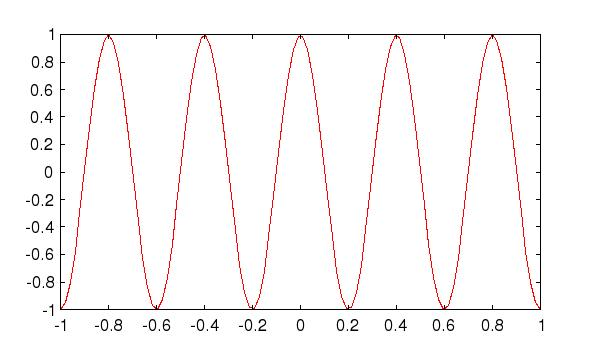
\includegraphics[width=8cm]{printfig1}}

